\documentclass[xcolor={dvipsnames,table}]{beamer}
\usepackage{epsfig,graphicx}
\usepackage{palatino}
\usepackage{fancybox}
\usepackage{relsize}
\usepackage[procnames]{listings}
\usepackage{hyperref}
\usepackage{qtree} % needed?
\usepackage{booktabs}
\usepackage{dirtree}
\usepackage[normalem]{ulem}
\usepackage{tikz}
\usetikzlibrary{arrows.meta,positioning,calc,fit,shapes.geometric,decorations.pathreplacing}


% fatter TT font
\renewcommand*\ttdefault{txtt}
% another TT, suggested by Alex
% \usepackage{inconsolata}
% \usepackage[T1]{fontenc} % needed as well?


\newcommand{\scale}{0.7}

\newcommand{\todo}[1]{{\emph{TODO: #1}}}
\newcommand{\martin}[1]{{\color{blue} Martin: #1}}
\newcommand{\abcdef}[1]{{\color{red} Author2: #1}}

% uncomment following for final submission
%\renewcommand{\todo}[1]{}
%\renewcommand{\martin}[1]{}
%\renewcommand{\author2}[1]{}

\newcommand{\code}[1]{{\texttt{#1}}}

\hypersetup{
  linkcolor  = black,
%  citecolor  = blue,
  urlcolor   = blue,
  colorlinks = true,
}

\beamertemplatenavigationsymbolsempty
\setbeamertemplate{footline}[frame number]





\newif\ifbook
\input{../shared/chisel}

% TikZ for diagrams
\usepackage{tikz}
\usetikzlibrary{positioning, arrows.meta}

% Optional visual tweaks
\tikzset{
    >=Stealth,
    every node/.style={rounded corners=2pt}
}

\title{Chisel and Simple Generators}
\author{Martin Schoeberl}
\date{\today}
\institute{Technical University of Denmark\\
Embedded Systems Engineering}

\begin{document}

\begin{frame}
\titlepage
\end{frame}

\begin{frame}[fragile]{TODO}
\begin{itemize}
\item Have the FBI story
\item Link the Scrum book
\item Repeat some Scala
\item Add stuff from xxx slides (e.g., pattern matching)
\end{itemize}
\end{frame}

\begin{frame}[fragile]{Motivating Example:\\
Lipsi: Probably the Smallest Processor in the World}
\begin{itemize}
\item Tiny processor
\item Simple instruction set
\item Shall be small
\begin{itemize}
\item Around 200 logic cells, one FPGA memory block
\end{itemize}
\item Hardware described in Chisel
\item Available at \url{https://github.com/schoeberl/lipsi}
\item Usage
\begin{itemize}
\item Utility processor for small stuff
% \item Could be used for your vending machine
\item In teaching introduction to computer architecture
\end{itemize}
\item The design took place on the island of Lipsi
\end{itemize}
\end{frame}

\begin{frame}[fragile]{The Design of Lipsi on Lipsi}
\begin{figure}
    \centering
    \includegraphics[scale=0.3]{../slides-tutorial/lipsi}
\end{figure}
\end{frame}

\begin{frame}[fragile]{Lipsi Implementation}
\begin{itemize}
\item Hardware described in Chisel
\item Tester in Chisel/Scala
\item Assembler in Scala
\begin{itemize}
\item Core case statement about 20 lines
\end{itemize}
\item Reference design of Lipsi as a software simulator in Scala
\item Testing:
\begin{itemize}
\item Self-testing assembler programs
\item Comparing hardware with a software simulator
\end{itemize}
\item All in a single programming language!
\item All in a single program
\item How much work is this?
\end{itemize}
\end{frame}

\begin{frame}[fragile]{Chisel is Productive}
\begin{itemize}
\item All coded and tested in less than 14 hours!
\end{itemize}
\begin{itemize}
\item The hardware in Chisel
\item Assembler in Scala
\item Some assembler programs (blinking LED)
\item Simulation in Scala
\item Two testers
\end{itemize}
\begin{itemize}
\item BUT, this does not include the design (done on paper)
\end{itemize}
\end{frame}

\begin{frame}[fragile]{Motivating Example: Lipsi, a Tiny Processor}
\begin{itemize}
\item Show in IntelliJ
\end{itemize}
\end{frame}

\begin{frame}[fragile]{Lecture 1}
\begin{itemize}
\item Waterfall and Agile design style
\item Quick overview of Chisel and Scala
\item Functional programming in Scala
\item Links to further reading and material
\end{itemize}
\end{frame}

% Week 1: Intro to Agile + Chisel

% --- Slide 1: Waterfall Model (Description) ---
\begin{frame}{The Classic Waterfall Model}
\begin{itemize}
    \item Traditional project management approach for software and hardware
    \item Development phases are sequential:
    \begin{enumerate}
        \item Requirements
        \item Design
        \item Implementation
        \item Verification
        \item Maintenance
    \end{enumerate}
    \item Each phase must be completed before moving to the next
    \item Changes are costly once early phases are complete
    \item I worked (long time ago) in such a team: was very boring
\end{itemize}
\end{frame}

\begin{frame}{Waterfall Model Diagram}
\centering
\resizebox{0.8\linewidth}{!}{%
\begin{tikzpicture}[
    node distance=1.4cm,
    every node/.style={draw, minimum width=3.2cm, minimum height=1.2cm, align=center}
]
\node[thick] (req) {Requirements};
\node[thick] (design) [below right=0.8cm and 0.6cm of req] {Design};
\node[thick] (impl) [below right=0.8cm and 0.6cm of design] {Implementation};
\node[thick] (verif) [below right=0.8cm and 0.6cm of impl] {Verification};
\node[thick] (maint) [below right=0.8cm and 0.6cm of verif] {Maintenance};

% Arrows
\draw[->, thick] (req.south east) -- (design.north west);
\draw[->, thick] (design.south east) -- (impl.north west);
\draw[->, thick] (impl.south east) -- (verif.north west);
\draw[->, thick] (verif.south east) -- (maint.north west);

% Feedback arrows
\draw[->, dashed, red] (design.west) .. controls +( -2,0) and +(-2,0) .. (req.west) node[midway,left]{Costly change};
\draw[->, dashed, red] (impl.west) .. controls +( -2,0) and +(-2,0) .. (design.west);
\draw[->, dashed, red] (verif.west) .. controls +( -2,0) and +(-2,0) .. (impl.west);

\end{tikzpicture}%
}
\end{frame}

% --- Slide 3: Waterfall Limitations ---
\begin{frame}{Limitations of the Waterfall Model}
\begin{itemize}
    \item Assumes requirements are fixed at the start
    \item Poor adaptability to changing customer needs
    \item Testing and feedback happen late in the process
    \item High risk of discovering major flaws late
    \item Not well-suited for rapid prototyping or exploratory projects
\end{itemize}
\end{frame}


\begin{frame}{Why Agile for Hardware?}
\begin{itemize}
    \item Traditional hardware development: long, rigid cycles
    \item Software has embraced Agile:
    \begin{itemize}
        \item Quick iterations
        \item Test-driven development
        \item Continuous integration
    \end{itemize}
    \item Hardware complexity is increasing $\rightarrow$ need for agility!
\end{itemize}
\end{frame}

\begin{frame}{Agile Iteration Cycle}
\centering
\resizebox{0.65\linewidth}{!}{%
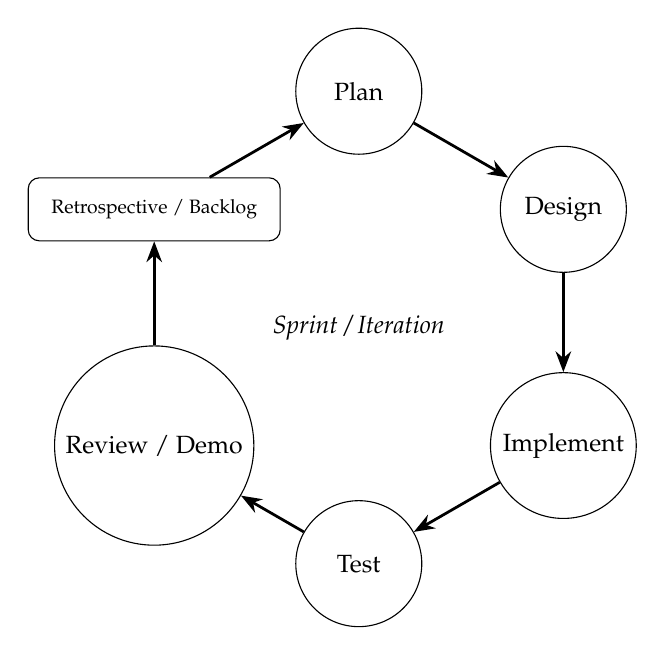
\begin{tikzpicture}[
  circular/.style={circle, draw, minimum size=1.6cm, font=\small, align=center},
  arrowstyle/.style={-Stealth, line width=1pt}
]
  % Place nodes in a circular layout
  \node[circular] (plan)      at (90:3cm)  {Plan};
  \node[circular] (design)    at (30:3cm)  {Design};
  \node[circular] (implement) at (-30:3cm) {Implement};
  \node[circular] (test)      at (-90:3cm) {Test};
  \node[circular] (review)    at (-150:3cm) {Review / Demo};
  \node[rectangle, draw, rounded corners, minimum width=3.2cm, minimum height=0.8cm, font=\scriptsize] (retro) at (-210:3cm) {Retrospective / Backlog};

  % Loop arrows
  \draw[arrowstyle] (plan) -- (design);
  \draw[arrowstyle] (design) -- (implement);
  \draw[arrowstyle] (implement) -- (test);
  \draw[arrowstyle] (test) -- (review);
  \draw[arrowstyle] (review) -- (retro);
  \draw[arrowstyle] (retro) -- (plan);

  % Central label
  \node at (0,0) [font=\small\itshape] {Sprint / Iteration};
\end{tikzpicture}%
}
\end{frame}
% --- Slide 1 ---
%\begin{frame}{Agile Iteration Phases (1/3)}
%\textbf{Plan}
%\begin{itemize}
%    \item Define goals for the upcoming sprint (typically 1-4 weeks)
%    \item Select features or fixes from the product backlog
%    \item Break down tasks into manageable user stories
%    \item Ensure each story has clear acceptance criteria
%\end{itemize}
%
%\medskip
%\textbf{Design}
%\begin{itemize}
%    \item Create a simple, implementable hardware design
%    \item Define interfaces and parameters
%    \item Update documentation and diagrams
%    \item Keep the design minimal to support fast iteration
%    \item Think: minimal viable product
%\end{itemize}
%\end{frame}
%
%% --- Slide 2 ---
%\begin{frame}{Agile Iteration Phases (2/3)}
%\textbf{Implement}
%\begin{itemize}
%    \item Write Chisel modules for new or updated functionality
%    \item Commit early and often to version control
%    \item Follow coding standards and naming conventions
%    \item Collaborate closely to avoid merge conflicts
%\end{itemize}
%
%\medskip
%\textbf{Test}
%\begin{itemize}
%    \item Use automated tests (e.g., \texttt{chiseltest}) to validate functionality
%    \item Run both unit tests and integration tests
%    \item Include corner cases and property-based checks
%    \item Maintain high test coverage throughout development
%\end{itemize}
%\end{frame}
%
%% --- Slide 3 ---
%\begin{frame}{Agile Iteration Phases (3/3)}
%\textbf{Review / Demo}
%\begin{itemize}
%    \item Present completed work to the team or stakeholders
%    \item Demonstrate working features in simulation or on FPGA
%    \item Gather feedback on design choices and implementation
%\end{itemize}
%
%\medskip
%\textbf{Retrospective / Backlog Refinement}
%\begin{itemize}
%    \item Reflect on what worked well and what can be improved
%    \item Adjust processes, tools, and team coordination as needed
%    \item Update the product backlog with new ideas or changes
%    \item Prepare for the next sprint cycle
%\end{itemize}
%\end{frame}

\begin{frame}{Hardware Design Today}
\begin{itemize}
    \item VHDL / Verilog = rigid, low-level
    \item Hard to reuse and test modularly
    \item Long simulation cycles
    \item Not optimized for iteration or testing early
    \item Often follows a version of the waterfall model
\end{itemize}
\end{frame}

\begin{frame}{Software-Inspired Hardware Flow}
\begin{enumerate}
    \item Write modular, parameterized designs
    \item Test-first using simulation
    \item Version control and continuous integration (CI)
    \begin{itemize}
\item For example, using GitHub actions
\end{itemize}
    \item Frequent review and refactor
    \begin{itemize}
\item With enough tests, refactoring is safe
\end{itemize}
    \item Code reviews and pull requests
\end{enumerate}
\end{frame}

\begin{frame}[fragile]{Chisel}
\begin{itemize}
\item A hardware \emph{construction} language
\begin{itemize}
\item Constructing Hardware in a Scala Embedded Language
\item If it compiles, it is synthesizable hardware 
\item Say goodbye to your unintended latches
\end{itemize}
\item Chisel is not a high-level synthesis language
\item Single source for two targets
\begin{itemize}
\item Cycle accurate simulation (testing)
\item Verilog for synthesis
\end{itemize}
\item Embedded in Scala
\begin{itemize}
\item Full power of Scala available
\item We use Scala to write the generators
\end{itemize}
\item Developed at UC Berkeley
\end{itemize}
\end{frame}

\begin{frame}[fragile]{The C Language Family}

\Tree[.C [
   [.{\bf Verilog} {\bf SystemVerilog} ]
   [.C++  \emph{SystemC}  ]
   [.Java [.Scala {\bf Chisel} ] ]
   [.C\# ] ] ]
 
\end{frame}

\begin{frame}[fragile]{Other Language Families}

\begin{columns}
\column{0.5\textwidth}
\begin{center}
\Tree[.Algol [.Ada [.{\bf VHDL} ] ] ]
\end{center}
\column{0.5\textwidth}
\begin{center}
\Tree[.Python [.{\bf MyHDL} ] ]
\end{center}
\end{columns}
\end{frame}

%\begin{frame}[fragile]{What Language do You Already Know?}
%\begin{itemize}
%\item ???
%\end{itemize}
%\end{frame}

\begin{frame}[fragile]{A Small Language}
\begin{itemize}
\item Chisel is a \emph{small} language
\item On purpose
\item Not many constructs to remember
\item The \href{https://github.com/freechipsproject/chisel-cheatsheet/releases/latest/download/chisel_cheatsheet.pdf}{Chisel Cheatsheet} fits on two pages
\item The power comes with Scala for circuit generators
\item With Scala, Chisel can grow with you
\end{itemize}
\end{frame}


%\begin{frame}[fragile]{Example: 2-bit Counter}
%\begin{verbatim}
%class Counter extends Module {
%  val io = IO(new Bundle {
%    val out = Output(UInt(2.W))
%  })
%  val count = RegInit(0.U(2.W))
%  count := count + 1.U
%  io.out := count
%}
%\end{verbatim}
%\end{frame}
%
%\begin{frame}[fragile]{Example Test}
%\begin{verbatim}
%test(new Counter) { c =>
%  c.io.out.expect(0.U)
%  c.clock.step()
%  c.io.out.expect(1.U)
%  c.clock.step()
%  c.io.out.expect(2.U)
%}
%\end{verbatim}
%\end{frame}



\begin{frame}[fragile]{Tool Flow for Chisel Defined Hardware}
\begin{figure}
    \centering
    \includegraphics[scale=0.35]{../figures/flow}
\end{figure}
\end{frame}

\begin{frame}[fragile]{Chisel is a Hardware Construction Language}
\begin{itemize}
\item The code looks much like Java code
\item But it is \emph{not} a program in the usual sense
\item It represents a circuit
\item The ``program'' constructs the circuit
\item All statements are ``executed'' in parallel
\item Statement order has \emph{mostly} no meaning
\end{itemize}
\end{frame}

\begin{frame}[fragile]{A Chisel Book}
\begin{figure}
    \centering
    \href{https://github.com/schoeberl/chisel-book}{\includegraphics[scale=0.4]{../cover-small}}
\end{figure}

\begin{itemize}
\item Available in open access (\href{https://www.imm.dtu.dk/~masca/chisel-book.pdf}{as PDF})
\begin{itemize}
\item Optimized for reading on a tablet (size, hyperlinks)
\end{itemize}
\item Amazon can do the printout
\end{itemize}
\end{frame}



\begin{frame}[fragile]{Chisel and Scala}
\begin{itemize}
\item Chisel is a library written in Scala
\begin{itemize}
\item Import the library with \code{import chisel3.\_}
\end{itemize}
\item Chisel code is Scala code
\item When it is run is \emph{generates} hardware
\begin{itemize}
\item Verilog for synthesis and siumulation
\end{itemize}
\item Chisel is an embedded domain-specific language
\item Two languages in one can be a little bit confusing
\end{itemize}
\end{frame}


\begin{frame}[fragile]{Scala}
\begin{itemize}
\item Object-oriented
\item Functional
\item Strongly typed with very good type inference
\item Runs on the Java virtual machine
\item Can call Java libraries
\item Consider it as Java++
\begin{itemize}
\item Can almost be written like Java
\item With a more lightweight syntax
\item Compiled to the JVM
\item Good Java interoperability
\item Many libraries available
\end{itemize}
\item \url{https://docs.scala-lang.org/tour/tour-of-scala.html}
\end{itemize}
\end{frame}

\begin{frame}[fragile]{Scala Hello World}
\begin{chisel}
object HelloWorld extends App {
  println("Hello, World!")
}
\end{chisel}
\begin{itemize}
\item Compile with \code{scalac} and run with \code{scala}
\item Or with \code{sbt run}
\item You can even use Scala as a scripting language
\item \code{scala-cli} is a generic Scala runner
\item Show both
\item Use \code{scala-cli} locally along the examples presented
\end{itemize}
\end{frame}


\begin{frame}[fragile]{Scala Values and Variables}
\begin{chisel}
// A value is a constant
val i = 0
// No new assignment; this will not compile
i = 3

// A variable can change the value
var v = "Hello"
v = "Hello World"

// Type usually inferred, but can be declared
var s: String = "abc"
\end{chisel}
\end{frame}

\begin{frame}[fragile]{Simple Loops}
\begin{chisel}
// Loops from 0 to 9
// Automatically creates loop value i
for (i <- 0 until 10) {
  println(i)
}
\end{chisel}
\end{frame}

\begin{frame}[fragile]{Conditions}
\begin{chisel}
for (i <- 0 until 10) {
  if (i%2 == 0) {
    println(i + " is even")
  } else {
    println(i + " is odd")
  }
}
\end{chisel}
\end{frame}

\begin{frame}[fragile]{Scala Arrays and Lists}
\begin{chisel}
// An integer array with 10 elements
val numbers = new Array[Integer](10)
for (i <- 0 until numbers.length) {
  numbers(i) = i*10
}
println(numbers(9))


// List of integers
val list = List(1, 2, 3)
println(list)
// Different form of list construction
val listenum = 'a' :: 'b' :: 'c' :: Nil
println(listenum)
\end{chisel}
\end{frame}


\begin{frame}[fragile]{Scala Classes}
\begin{chisel}
// A simple class
class Example {
  // A field, initialized in the constructor
  var n = 0
  
  // A setter method
  def set(v: Integer) = {
    n = v
  }
  
  // Another method
  def print() = {
    println(n)
  }
}
\end{chisel}
\end{frame}

\begin{frame}[fragile]{Scala (Singleton) Object}
\begin{chisel}
object Example {}
\end{chisel}
\begin{itemize}
\item For \emph{static} fields and methods
\begin{itemize}
\item Scala has no static fields or methods like Java
\end{itemize}
\item Needed for \code{main}
\item Useful for helper functions
\end{itemize}
\end{frame}

\begin{frame}[fragile]{Tuples}
\begin{itemize}
\item Scala has the notion of tuples
\item Can hold a sequence of different types
\item Fields are then accessed with \code{.\_n}, starting with 1
\item Easy option to return more than one value from a function
\end{itemize}
\shortlist{../code/scala_tuple.txt}
\end{frame}

\begin{frame}[fragile]{Scala Collections}
\begin{itemize}
\item Scala has a powerful \href{https://docs.scala-lang.org/overviews/collections-2.13/overview.html}{collection library}
\item \code{Seq} is an ordered collection of elements (also called a sequence)
\item The default implementation is immutable
\item We index into a \code{Seq} with \code{()}, with zero-based indexing.
\end{itemize}
\shortlist{../code/scala_seq.txt}
\end{frame}

\begin{frame}[fragile]{Functional Programming}
\begin{itemize}
\item Functional programming (FP) treats computation as the evaluation of functions
\item Functions are first-class objects
\item Can be a parameter of a function
\item Can be returned from a function
\item Avoid mutable state
\item Recursion is \emph{not} the main point of FP
\item Higher-order functions take functions as arguments
\end{itemize}
\end{frame}


\begin{frame}[fragile]{First-Class Functions}
\begin{itemize}
    \item In Scala, functions can be assigned to variables, passed as arguments, or returned
\end{itemize}

\begin{verbatim}
// A normal function definition
def double(x: Int): Int = x * 2

println(double(5))   // prints 10

// A function that takes another function
def applyTwice(f: Int => Int, v: Int): Int = {
  f(f(v))
}

println(applyTwice(double, 3)) // prints 12
\end{verbatim}
\end{frame}

\begin{frame}[fragile]{Function Literals (Anonymous Functions)}
\begin{itemize}
    \item A function literal is a shorthand for defining a function "inline"
    \item by the \code{=>} symbol
    \item Does not require a name (\texttt{def})
    \item Often used with higher-order functions
\end{itemize}

\begin{verbatim}
// Normal function
def square(x: Int): Int = x * x

// Function literal (anonymous function)
val squareFn = (x: Int) => x * x

// Using a literal directly
val nums = List(1, 2, 3, 4)
val squares = nums.map(x => x * x)
println(squares) // List(1, 4, 9, 16)
\end{verbatim}
\end{frame}

% --- Slide 3 ---
\begin{frame}[fragile]{Higher-Order Functions}
\begin{itemize}
    \item Functions that take other functions as arguments
    \item What we just used before
    \item Useful for hardware generators (map, filter, etc.)
\end{itemize}

\begin{verbatim}
val nums = List(1, 2, 3, 4)
val squares = nums.map(x => x * x)
println(squares) // List(1, 4, 9, 16)
\end{verbatim}

%\begin{itemize}
%    \item This is similar to generating a Vec of wires in Chisel:
%\end{itemize}
%
%\begin{verbatim}
%val wires = VecInit(Seq.fill(4)(Wire(UInt(8.W))))
%\end{verbatim}
\end{frame}

% --- Slide 4 ---
\begin{frame}[fragile]{Immutability}
\begin{itemize}
    \item FP encourages immutable values (using \texttt{val})
    \item No side effects: easier to reason about hardware generation
\end{itemize}

\begin{verbatim}
val a = 5
// a = 6   // ERROR: reassignment not allowed

val b = a + 1   // OK, creates a new value
\end{verbatim}

\begin{itemize}
    \item In Chisel, \texttt{val} describes structure, not time-varying state
    \item Registers (\texttt{Reg}) are explicit when you need mutable hardware state
\end{itemize}
\end{frame}

% --- Slide 5 ---
%\begin{frame}[fragile]{Pure Functions}
%\begin{itemize}
%    \item A pure function:
%    \begin{itemize}
%        \item Always returns the same output for the same input
%        \item Has no side effects
%    \end{itemize}
%\end{itemize}
%
%\begin{verbatim}
%def add(a: Int, b: Int): Int = a + b
%\end{verbatim}
%
%\begin{itemize}
%    \item Combinational hardware modules are pure
%    \item Side effects (state, IO, randomness) are controlled explicitly
%\end{itemize}
%\end{frame}

% --- Slide 6 ---
\begin{frame}[fragile]{Mapping Over Collections}
\begin{itemize}
    \item \texttt{map} applies a function to each element of a collection
    \item Produces a new collection of the same size
\end{itemize}

\begin{verbatim}
val nums = List(1, 2, 3, 4)
def square(x: Int): Int = x * x

val squares = nums.map(square)
println(squares) // List(1, 4, 9, 16)
\end{verbatim}

\end{frame}

% --- Slide 7 ---
\begin{frame}[fragile]{Filtering Collections}
\begin{itemize}
    \item \texttt{filter} keeps only elements that satisfy a condition
\end{itemize}

\begin{verbatim}
val nums = List(1, 2, 3, 4, 5, 6)

def isEven(x: Int): Boolean = (x % 2 == 0)
val evens = nums.filter(isEven)

println(evens) // List(2, 4, 6)
\end{verbatim}

\end{frame}

% --- Slide 8 ---
\begin{frame}[fragile]{Reducing Collections}
\begin{itemize}
    \item \texttt{reduce} combines all elements using a binary function
    \item Useful for sums, products, and combining signals
\end{itemize}

\begin{verbatim}
val nums = List(1, 2, 3, 4)

def add(x: Int, y: Int): Int = x + y
val sum = nums.reduce(add)

println(sum) // 10
\end{verbatim}

\begin{itemize}
    \item Hardware analogy: adding a set of signals
    \item Use \code{reduceTree} for a balanced reduction tree
\end{itemize}
\end{frame}



\begin{frame}[fragile]{Scala Build Tool (sbt)}
\begin{itemize}
\item Downloads Scala compiler if needed
\item Downloads dependent libraries (e.g., Chisel)
\item Compiles Scala programs
\item Executes Scala programs
\item Does a lot of magic, maybe too much
\item Compile and run with:
\end{itemize}
\begin{chisel}
sbt run
\end{chisel}
\end{frame}

\begin{frame}[fragile]{File Organization in Scala/Chisel}
\dirtree{%
.1 project.
.2 src.
.3 main.
.4 scala.
.5 package.
.6 sub-package.
.3 test.
.4 scala.
.5 package.
.2 target.
.2 generated.
}
\end{frame}



\begin{frame}[fragile]{ScalaTest}
\begin{itemize}
\item Testing framework for Scala and Java
\item \code{sbt} understands ScalaTest
\item Add library to \code{build.sbt}
\begin{chisel}
libraryDependencies += "org.scalatest" %% "scalatest" % "3.1.4" % "test"
\end{chisel}
\item Run all tests with:
\begin{chisel}
sbt test
\end{chisel}
\item When all (unit) tests are ok, the test passes
\item A little bit funny syntax
\item ChiselTest is based on ScalaTest
\end{itemize}
\end{frame}

\begin{frame}[fragile]{ScalaTest Hello World}
\shortlist{../code/scalatest_hello_world.txt}
\end{frame}


\begin{frame}[fragile]{Further Reading and Web Resources}
\begin{itemize}
\item \href{https://www.sciencedirect.com/science/article/pii/S014193312500050X}{Scala defined hardware generators for Chisel}
\begin{itemize}
\item Journal article with generator examples
\end{itemize}
\item \href{http://www.imm.dtu.dk/~masca/chisel-book.html}{Chisel book website}
\begin{itemize}
\item Information on Chisel, a bit of Scala
\item Download the free PDF
\end{itemize}
\item \href{http://www2.imm.dtu.dk/courses/02139/}{Digital design course at DTU}
\begin{itemize}
\item Slides on digital design with Chisel
\end{itemize}
\item \href{https://github.com/schoeberl/chisel-lab}{Digital design lab at DTU}
\begin{itemize}
\item Lab material for the digital design course
\item Option to train a bit on Chisel
\end{itemize}
\end{itemize}
\end{frame}


\begin{frame}[fragile]{Lab 1}
\begin{itemize}
\item I assume that you installed all tools and did lab0 as homework
\item Functional programming in Scala
\item The lab contains tests, run with \code{sbt test}
\item Code is in \href{https://github.com/schoeberl/agile-hw/tree/main/lab1}{lab1}
\end{itemize}
\end{frame}

\begin{frame}[fragile]{Lecture 2}
\begin{itemize}
\item Introduction to Chisel
\item Functional programming for generators
\end{itemize}
\end{frame}

\begin{frame}[fragile]{Chisel in Scala}
\begin{itemize}
\item Chisel components are Scala classes
\item Chisel code is in the constructor
\item Executed at object creation time
\item Builds the network of hardware objects
\item Testers are written in Scala to drive the tests
\end{itemize}
\end{frame}



\begin{frame}[fragile]{Chisel Data Types}
\begin{itemize}
\item Data types for values on wires or state elements
\item Raw collection of bits is type \code{Bits}
\item Simple types to represent integer numbers
\begin{itemize}
\item Unsigned: \code{UInt}
\item Signedigned: \code{SInt}
\item Subtype of \code{Bits}
\end{itemize}
\item Automatic bit width inference
\item Boolean values are of type \code{Bool}, a single bit value
\item \emph{Interesting} way to specify constants
\end{itemize}
\begin{chisel}
1.U
"habcd".U
"b0101".U
-5.S
true.B
\end{chisel}
\end{frame}

\begin{frame}[fragile]{Chisel Data Types}
\begin{itemize}
\item Bit width can be explicitly specified with a width type
\begin{itemize}
\item \code{SInt} will be sign extended
\item \code{UInt} will be zero extended
\end{itemize}
\end{itemize}
\begin{chisel}
UInt(8.W)
SInt(16.W)
0.U(32.W)
"habcd".U(24.W)
-5.S(16.W)
\end{chisel}
\begin{itemize}
\item Chisel data types are different from Scala builtin types (e.g., Scala's \code{Int})
\end{itemize}
\end{frame}

\begin{frame}[fragile]{Bitwise Logical Operations}
\begin{itemize}
\item Bitwise NOT, AND, OR, and XOR
\item Automatic size extension to larger operand
\end{itemize}
\begin{chisel}
val notVal = ~x
val maskOut = x & "b00001111".U
val orVal = x | y
val xorVal = x ^ y
\end{chisel}
\begin{itemize}
\item Bit reduction
\item Results in a single bit
\end{itemize}
\begin{chisel}
x.andR
x.orR
x.xorR
\end{chisel}
\end{frame}

\begin{frame}[fragile]{Arithmetic Operations}
\begin{itemize}
\item Addition, subtraction, multiplication, division, modulos
\item Automatic size extension to larger operand
\end{itemize}
\begin{chisel}
+, -, *, /, %
\end{chisel}
\begin{itemize}
\item Left and right shifts
\item Left shift extends bit width
\item Right shift reduces bit width
\end{itemize}
\begin{chisel}
<<, >>
\end{chisel}
\end{frame}

%\begin{frame}[fragile]{Bitfield Manipulations}
%\begin{itemize}
%\item Extract a single bit
%\end{itemize}
%\begin{chisel}
%val sign = x(31)
%\end{chisel}
%\begin{itemize}
%\item Extract a sub field from end to start position
%\end{itemize}
%\begin{chisel}
%val lowByte = word(7, 0)
%\end{chisel}
%\begin{itemize}
%\item Concatenate bit fields
%\end{itemize}
%\begin{chisel}
%val word = Cat(highByte, lowByte)
%\end{chisel}
%\end{frame}

\begin{frame}[fragile]{Comparison}
\begin{itemize}
\item The usual operations
\begin{itemize}
\item Unusual equal and unequal operator symbols
\item To keep the original Sala operators usable for references
\end{itemize}
\item Operands are \code{UInt} and \code{SInt}
\item Operands can be \code{Bool} for equal and unequal
\item Result is \code{Bool}
\end{itemize}
\begin{chisel}
===, =/=
>, >=, <, <=
\end{chisel}
\end{frame}

\begin{frame}[fragile]{Boolean Logical Operations}
\begin{itemize}
\item Operands and result are \code{Bool}
\item Logical NOT, AND, and OR
\end{itemize}
\begin{chisel}
val notX = !x
val bothTrue = a && b
val orVal = x || y
\end{chisel}
\end{frame}

\begin{frame}[fragile]{Combinational Circuits}
\begin{itemize}
\item Circuit is a graph of nodes
\item A node is a hardware operator with zero or more inputs
\item Textual expression to wire up nodes
\item Named wires with some (unspecified) width
\end{itemize}
\begin{chisel}
(a | b) & ~c
\end{chisel}
\end{frame}

\begin{frame}[fragile]{Combinational Circuits}
\begin{itemize}
\item Simple expressions represent a circuit tree
\item Arbitrary directed acyclic graphs need named subexpressions
\item Using Scala's \code{val} keyword for variables that don't change
\item Referenced multiple times
\end{itemize}
\begin{chisel}
val cond = a & b
val result = (cond & selA) | (!cond & selB)
\end{chisel}
\end{frame}

\begin{frame}[fragile]{Connections}
\begin{itemize}
\item Connections with the \code{:=} assignment
\item When \emph{reassigning} a value to a wire, port, or register
\begin{chisel}
  adder.io.a := ina
  adder.io.b := inb
\end{chisel}
%\item Automatic bulk connections between components
%\begin{chisel}
%  dec.io <> exe.io
%  mem.io <> exe.io
%\end{chisel}
\end{itemize}
\end{frame}


\begin{frame}[fragile]{Register}
\begin{itemize}
\item State elements
\item Has it's own Chisel type \code{Reg}
\item Positive edge triggered D flip-flop
\item Synchronous reset
\item Clock and reset are \emph{hidden wires}
\end{itemize}
\begin{chisel}
val q = RegNext(d)
\end{chisel}
\begin{itemize}
\item \code{d} is the input, \code{q} the output
\item Register type is inferred by the input (d) type
\end{itemize}
\end{frame}

\begin{frame}[fragile]{Register}
\begin{itemize}
\item Reset value as parameter on a \code{RegInit} constructor
\end{itemize}
\begin{chisel}
val initReg = RegInit(0.U(8.W))
\end{chisel}
\begin{itemize}
\item With this forward declaration we later assign the input
\end{itemize}
\begin{chisel}
initReg := initReg + 1.U
\end{chisel}
\begin{itemize}
\item A register can also be defined within an expression
\end{itemize}
\shortlist{../code/sequ_reg_rising.txt}
\end{frame}


\begin{frame}[fragile]{A Multiplexer}
\begin{figure}
  \includegraphics[scale=\scale]{../figures/mux}
\end{figure}
\begin{itemize}
\item A Multiplexer selects between alternatives
\item So common that Chisel provides a construct for it
\item Selects \code{a} when \code{sel} is \code{true.B} otherwise \code{b}
\item Could be implemented with conditional updates
\item Automagical type selection on input types
\end{itemize}
\shortlist{../code/mux.txt}
\end{frame}

%\begin{frame}[fragile]{Expressions are Combinational Circuits}
%\begin{chisel}
%(a | b) & ~(c ^ d)
%
%val addVal = a + b
%val orVal = a | b
%val boolVal = a >= b
%\end{chisel}
%\begin{itemize}
%\item The usual operations 
%\item Simple name assignment with val
%\item Width inference
%\item Type inference
%\item Types: Bits, UInt, SInt, Bool
%\end{itemize}
%\end{frame}

\begin{frame}[fragile]{Conditional Updates for Combinational Circuits}
\shortlist{../code/comb_elsewhen.txt}
\begin{itemize}
\item Similar to VHDL \code{process} or SystemVerilog \code{always\_comb}
\item Chisel checks for complete assignments in all branches
\item Latches give compile error
\end{itemize}
\end{frame}

\begin{frame}[fragile]{Chained Conditionals}
\begin{itemize}
\item Chain of conditionals with \code{.elsewhen}
\item With an optional \emph{else} path with \code{.otherwise}
\item Note that Scala has \code{if/else}
\begin{itemize}
\item Does NOT result in hardware
\item Are used to conditionally \emph{generate} hardware
\item We will look at this later
\end{itemize}
\item Note the ``.'' at the operators
\end{itemize}
\begin{chisel}
  when (c1) { v := 1.U }
  .elsewhen (c2) { v := 2.U }
  .otherwise { v := 3.U }
\end{chisel}
\end{frame}

\begin{frame}[fragile]{Switch Statement}
\begin{itemize}
\item Series of comparisons
\item Chisel allows combinational logic be updated conditionally 
\item Chisel disallows incomplete specified logic (= latches)
\item Chisel will report a runtime error
\end{itemize}
\begin{chisel}
  switch(fn) {
    is(0.U) { result := a + b }
    is(1.U) { result := a - b }
    is(2.U) { result := a | b }
    is(3.U) { result := a & b }
  }
\end{chisel}
\end{frame}


\begin{frame}[fragile]{Data Aggregation with Bundles}
\begin{itemize}
\item A \code{Bundle} groups several named fields
\item Like a C struct or VHDL record
\item \code{Vec} is a vector of elements with the same type
\item Can be arbitrary mixed
\end{itemize}
\begin{chisel}
class AluFields extends Bundle {
  val function = UInt(2.W)
  val inputA = UInt(8.W)
  val inputB = UInt(8.W)
  val result = UInt(8.W)
}
\end{chisel}
\end{frame}

\begin{frame}[fragile]{Vectors}
\begin{itemize}
\item Indexable vector of elements
\item Elements can be Chisel basic elements, or bundles
\item Type is specified as second parameter
\end{itemize}
\begin{chisel}
val myVec = Vec(3, SInt(10.W))
val y = myVec(2)
myVec(0) := -3.S
\end{chisel}
\begin{itemize}
\item A register file as a register of a vector
\end{itemize}
\begin{chisel}
val vecReg = Reg(Vec(32, SInt(32.W)))
\end{chisel}
\end{frame}

\begin{frame}[fragile]{IO Ports}
\begin{chisel}
class Channel extends Bundle {
  val data = Input(UInt(8.W))
  val ready = Output(Bool())
  val valid = Input(Bool())
}
\end{chisel}
\begin{itemize}
\item Ports are Bundles with directions
\item Ports are used to connect modules
\item Can be reversed with the \code{Flipped}
\item Convenient to have one bundle definition working as a source
and the destination used between two modules
\end{itemize}
\begin{chisel}
class ChannelUsage extends Bundle {
  val input = new Channel()
  val output = Flipped(new Channel())
}
\end{chisel}
\end{frame}


\begin{frame}[fragile]{Modules}
\begin{itemize}
\item Modules are used to organize the circuit
\item Similar to VHDL components (entity/architecture)
\item A class that inherits from \code{Module}
\item Circuit description in the constructor
\item Interface (port) is a \code{Bundle}, wrapped into an \code{IO()}, and stored in the field \code{io}
\end{itemize}
\begin{chisel}
class Adder extends Module {
  val io = IO(new Bundle {
    val a = Input(UInt(4.W))
    val b = Input(UInt(4.W))
    val result = Output(UInt(4.W))
  })

  val addVal = io.a + io.b
  io.result := addVal
}
\end{chisel}
\end{frame}

\begin{frame}[fragile]{Module Usage}
\begin{itemize}
\item Create with \code{new} and wrap into a \code{Module()}
\item Interface port via the \code{io} field
\item Note the assignment operator \code{:=} on \code{io} fields
\end{itemize}
\begin{chisel}
  val adder = Module(new Adder())
  adder.io.a := ina
  adder.io.b := inb
  val result = adder.io.result
\end{chisel}
\end{frame}

%\begin{frame}[fragile]{A Small Circuit}
%\begin{itemize}
%\item Our Chisel knowledge is complete enough\\ to implement any digital circuit
%\item Maybe not in the most elegant way ;-)
%\item A counter is a simple basic component
%\item The following counts form 0 to 100
%\end{itemize}
%\begin{chisel}
%  val cntReg = RegInit(0.U(8.W))
%
%  cntReg := Mux(cntReg === 100.U,
%    0.U, cntReg + 1.U)
%\end{chisel}
%\end{frame}
%
%\begin{frame}[fragile]{The Complete Counter Module}
%\begin{chisel}
%class Counter extends Module {
%  val io = IO(new Bundle {
%    val cnt = Output(UInt(8.W))
%  })
%
%  val cntReg = RegInit(0.U(8.W))
%
%  cntReg := Mux(cntReg === 100.U,
%    0.U, cntReg + 1.U)
%
%  io.cnt := cntReg
%}
%\end{chisel}
%\end{frame}

\begin{frame}[fragile]{Hello World in Chisel}
\shortlist{../code/hello.txt}
\end{frame}

\begin{frame}[fragile]{Chisel Main}

\begin{itemize}
\item Create one top-level Module
\item Invoke the Verilog emitter from the Scala \code{main} (or App)
\item Following code generates Verilog code
\end{itemize}
\shortlist{../code/generate.txt}
\end{frame}

\begin{frame}[fragile]{Time for a Break}
\begin{itemize}
\item We need some coffee and sweet stuff
\end{itemize}
\end{frame}

%\begin{frame}[fragile]{Generic Components}
%\begin{chisel}
%val c = Mux(cond, a, b)
%\end{chisel}
%\begin{itemize}
%\item This is a multiplexer
%\item Input can be any type
%\end{itemize}
%\end{frame}

\begin{frame}[fragile]{Functions}
\begin{itemize}
\item Circuits can be encapsulated in functions
\item Each \emph{function call} generates hardware
\item Simple functions can be a single line
\end{itemize}
\begin{chisel}
  def adder(v1: UInt, v2: UInt) = v1 + v2
  
  val add1 = adder(a, b)
  val add2 = adder(c, d)
\end{chisel}
\end{frame}

\begin{frame}[fragile]{Functional Abstraction}
\begin{chisel}
  def addSub(add: Bool, a: UInt, b: UInt) =
    Mux(add, a+b, a-b)

  val res = addSub(cond, a, b)
  
  def rising(d: Bool) = d && !RegNext(d)
\end{chisel}
\begin{itemize}
\item Functions for repeated pieces of logic
\item May contain state
\item Functions may return \emph{hardware}
\end{itemize}
\end{frame}

\begin{frame}[fragile]{The Counter as a Function}
\begin{itemize}
\item Longer functions in curly brackets
\item Last value is the return value
\end{itemize}
\begin{chisel}
def counter(n: UInt) = {
  
  val cntReg = RegInit(0.U(8.W))
  
  cntReg := cntReg + 1.U
  when(cntReg === n) {
    cntReg := 0.U
  }
  cntReg
}

val counter100 = counter(100.U)
\end{chisel}
\end{frame}


%\begin{frame}[fragile]{Functions}
%\begin{itemize}
%\item Example from Patmos execute stage
%\end{itemize}
%\begin{chisel}
%def alu(func: Bits, op1: UInt, op2: UInt): Bits = {
%  val result = UInt(width = DATA_WIDTH)
%  // some more lines...
%  switch(func) {
%    is(FUNC_ADD) { result := sum }
%    is(FUNC_SUB) { result := op1 - op2 }
%    is(FUNC_XOR) { result := (op1 ^ op2).toUInt }
%    // some more lines
%  }
%  result
%}
%\end{chisel}
%\end{frame}




\begin{frame}[fragile]{Use Functional Programming for Generators}
\shortlist{../code/fun_first.txt}
\shortlist{../code/fun_func_lit.txt}
\shortlist{../code/fun_reduce_tree.txt}
\begin{itemize}
\item This is a simple example
\item What about an arbitration tree with fair arbitration?
\end{itemize}
\end{frame}

\begin{frame}[fragile]{Functional Generation}
\begin{itemize}
\item Anonymous functions, called \emph{function literal}
\begin{chisel}
  (param) => function body
\end{chisel}
\item A function for a minimum search
\shortlist{../code/fun_min.txt}
\end{itemize}
\end{frame}

%\begin{frame}[fragile]{Minimal Function with Index}
%\begin{itemize}
%\item Was the example for Tjark's heap sort
%\shortlist{../code/fun_min2.txt}
%\item We need an extra bundle to hold both values
%\item A for loop is not so functional
%\end{itemize}
%\end{frame}
%
%\begin{frame}[fragile]{We Can Use Tuples and zipWithIndex}
%\begin{itemize}
%\item \code{zipWithIndex} transforms the original sequence to a sequence of tuples
%with second element is the index
%\item Use \code{map} to translate from Scala \code{Int} to Chisel \code{UInt}
%\item \code{reduce} does the minimum function, actually called 2 times (we could optimize this)
%\shortlist{../code/fun_min3.txt}
%\item The result is a Scala \code{Vector} and not a Chisel \code{Vec}
%\end{itemize}
%\end{frame}
%
%\begin{frame}[fragile]{Solution with a Vec}
%\begin{itemize}
%\item This results in a Chisel \code{Vec}
%\shortlist{../code/fun_min4.txt}
%\item
%\item We should add a \code{reduceTree} to the Scala sequence version (\code{TraversableOnce})
%\end{itemize}
%\end{frame}

%\begin{frame}[fragile]{An Arbiter}
%\shortlist{../code/fun_arbiter.txt}
%\end{frame}

\begin{frame}[fragile]{Testing with Chisel}
\begin{itemize}
\item A test contains:
\begin{itemize}
\item a device under test (DUT) and
\item the testing logic
\end{itemize}
\item Set input values with \code{poke}
\item Advance the simulation with \code{step}
\item Read the output values with \code{peek}
\item Compare the values with \code{expect}
\item Import following packages:
\shortlist{../code/test_import.txt}
\end{itemize}
\end{frame}

\begin{frame}[fragile]{An Example DUT}
\begin{itemize}
\item A device-under test (DUT)
\item Just 2-bit AND logic
\shortlist{../code/test_dut.txt}
\end{itemize}
\end{frame}

\begin{frame}[fragile]{A ChiselTest}
\begin{itemize}
\item Extends class \code{AnyFlatSpec} with \code{ChiselScalatestTester}
\item Has the device-under test (DUT) as parameter of the \code{test} function
\item Test function contains the test code
\item Testing code can use all features of Scala
\end{itemize}
\end{frame}

%\begin{frame}[fragile]{A Simple Tester}
%\begin{itemize}
%\item Just using \code{println} for manual inspection
%\shortlist{../code/test_bench_simple.txt}
%\end{itemize}
%\end{frame}


\begin{frame}[fragile]{A Test}
\begin{itemize}
\item Poke values and \code{expect} some output
\shortlist{../code/test_bench.txt}
\end{itemize}
\end{frame}

%\begin{frame}[fragile]{Testing}
%\begin{itemize}
%\item Within Chisel with a tester (= Scala program)
%\item May include waveform generation
%\item peek and poke to read and set values
%\begin{itemize}
%\item Remember the BASIC days ;-)
%\end{itemize}
%\item printf in simulation on rising edge
%\begin{chisel}
%printf("Counting %x\n", r1)
%\end{chisel}
%\end{itemize}
%\end{frame}
%
%\begin{frame}[fragile]{Testing Example}
%\shortlist{../code/test_bench_simple.txt}
%\end{frame}


\begin{frame}[fragile]{Lab 2}
\begin{itemize}
\item Write a search for the maximum circuit (with \code{treeReduce()})
\item Optional: add the generation of the index of the maximum value
\item Emit Verilog with \code{emitVerilog(new Comp())}, so you can synthesize it at the Thursday session
\item Code is in \href{https://github.com/schoeberl/agile-hw/tree/main/lab2}{lab2}
\end{itemize}
\end{frame}

\begin{frame}[fragile]{Lecture 3}
\begin{itemize}
\item Hardware generators
\item Object-oriented hardware design
\end{itemize}
\end{frame}


\begin{frame}[fragile]{Scala List for Enumeration}
\begin{chisel}
  val empty :: full :: Nil = Enum(2)
\end{chisel}
\begin{itemize}
\item Can be used in wires and registers
\item Symbols for a state machine
\end{itemize}
\end{frame}

\begin{frame}[fragile]{Finite State Machine}
\begin{chisel}
  val empty :: full :: Nil = Enum(2)
  val stateReg = RegInit(empty)
  val dataReg = RegInit(0.U(size.W))

  when(stateReg === empty) {
    when(io.enq.write) {
      stateReg := full
      dataReg := io.enq.din
    }
  }.elsewhen(stateReg === full) {
    when(io.deq.read) {
      stateReg := empty
    }
  }
\end{chisel}
\begin{itemize}
\item A simple buffer for a bubble FIFO
\end{itemize}
\end{frame}

\begin{frame}[fragile]{Component Generation}
\begin{chisel}
val cores = new Array[Module](32)

for (j <- 0 until 32)
  cores(j) = Module(new CPU())
\end{chisel}
\begin{itemize}
\item Use Scala array to collect components
\item Generation with a Scala loop
\end{itemize}
\end{frame}

\begin{frame}[fragile]{Logic Generation}
\begin{itemize}
\item Read a file into a table
\begin{itemize}
\item E.g., to read in ROM content for a processor
\end{itemize}
\item Generate a truth table algorithmically
\begin{itemize}
\item E.g., generate binary to BCD translation
\end{itemize}
\item Use the full power of Scala
\end{itemize}
\begin{chisel}
val byteArray = Files.readAllBytes(Paths.get(fileName))
val arr = new Array[Bits](byteArray.length)
for (i <- 0 until byteArray.length) {
  arr(i) = Bits(byteArray(i), 8)
}
val rom = Vec[Bits](arr)
\end{chisel}
\end{frame}

\begin{frame}[fragile]{Parameterization}
\begin{chisel}
class ParamChannel(n: Int) extends Bundle {
  val data = Input(UInt(n.W))
  val ready = Output(Bool())
  val valid = Input(Bool())
}

val ch32 = new ParamChannel(32)
\end{chisel}
\begin{itemize}
\item Bundles and modules can be parametrized
\item Pass a parameter in the constructor
\end{itemize}

\end{frame}
\begin{frame}[fragile]{A Module with a Parameter}
\begin{chisel}
class ParamAdder(n: Int) extends Module {
  val io = IO(new Bundle {
    val a = Input(UInt(n.W))
    val b = Input(UInt(n.W))
    val result = Output(UInt(n.W))
  })

  val addVal = io.a + io.b
  io.result := addVal
}

val add8 = Module(new ParamAdder(8))
\end{chisel}
\begin{itemize}
\item Parameter can also be a Chisel type
\item Can also be a generic type:
\item \code{class Mod[T <: Bits](param: T) extends...}
\end{itemize}
\end{frame}

\begin{frame}[fragile]{Scala \code{for} Loop for Circuit Generation}
\begin{chisel}
val shiftReg = RegInit(0.U(8.W))

shiftReg(0) := inVal

for (i <- 1 until 8) {
  shiftReg(i) := shiftReg(i-1)
}
\end{chisel}
\begin{itemize}
\item \code{for} is Scala
\item This loop generates several connections
\item The connections are parallel hardware
\end{itemize}
\end{frame}

\begin{frame}[fragile]{Conditional Circuit Generation}
\begin{chisel}
class Base extends Module { val io = new Bundle() }
class VariantA extends Base { }
class VariantB extends Base { }

val m = if (useA) Module(new VariantA())
        else Module(new VariantB())
\end{chisel}
\begin{itemize}
\item \code{if} and \code{else} is Scala
\item \code{if} is an expression that returns a value
\begin{itemize}
\item Like ``\code{cond ? a : b;}'' in C and Java
\end{itemize}
\item This is not a hardware multiplexer
\item Decides which module to generate
\item Could even read an XML file for the configuration
\end{itemize}
\end{frame}

% use this for the 4 unit version
\begin{frame}[fragile]{Chisel has a Multiplexer}
\begin{figure}
  \includegraphics[scale=\scale]{../figures/mux}
\end{figure}
\shortlist{../code/mux.txt}
\begin{itemize}
\item So what?
\item Wait... What type is \code{a} and \code{b}?
\begin{itemize}
\item Can be any Chisel type!
\end{itemize}
\end{itemize}
\end{frame}

\begin{frame}[fragile]{Chisel has a Generic Multiplexer}
\begin{figure}
  \includegraphics[scale=\scale]{../figures/mux}
\end{figure}
\shortlist{../code/mux.txt}
\begin{itemize}
\item SW people may not be impressed
\item They have generics since Java 1.5 in 2004
\begin{itemize}
\item \code{List<Flowers> != List<Cars>}
\end{itemize}
\end{itemize}
\end{frame}


\begin{frame}[fragile]{Generics in Hardware Construction}
\begin{itemize}
\item Chisel supports generic classes with type parameters
\item Write hardware generators independent of concrete type
\item This is a multiplexer \emph{generator}
\end{itemize}
\shortlist{../code/param_func.txt}
\end{frame}

\begin{frame}[fragile]{Put Generics Into Use}
\begin{itemize}
\item Let us implement a generic FIFO
\item Use the generic ready/valid interface from Chisel
\end{itemize}
\shortlist{../code/fifo_decoupled.txt}
\end{frame}

\begin{frame}[fragile]{Define the FIFO Interface}
\shortlist{../code/fifo_io.txt}
\begin{itemize}
\item We need enqueueing and dequeueing ports
\item Note the \code{Flipped}
\begin{itemize}
\item It switches the direction of ports
\item No more double definitions of an interface
\end{itemize}
\end{itemize}
\end{frame}

\begin{frame}[fragile]{But What FIFO Implementation?}
\begin{itemize}
\item Bubble FIFO (good for low data rate)
\item Double buffer FIFO (fast restart)
\item FIFO with memory and pointers (for larger buffers)
\begin{itemize}
\item Using flip-flops
\item Using on-chip memory
\end{itemize}
\item And some more...
\end{itemize}
\begin{itemize}
\item This calls for object-oriented \sout{programming} \emph{hardware construction}
\end{itemize}
\end{frame}

\begin{frame}[fragile]{Abstract Base Class and Concrete Extension}
\shortlist{../code/fifo_abstract.txt}
\begin{itemize}
\item May contain common code
\item Extend by concrete classes
\end{itemize}
\begin{chisel}
class BubbleFifo[T <: Data](gen: T, depth: Int) extends Fifo(gen: T, depth: Int) {
\end{chisel}
\end{frame}



\begin{frame}[fragile]{Select a Concrete FIFO Implementation}
\begin{itemize}
\item Decide at hardware generation
\item Can use all Scala/Java power for the decision
\begin{itemize}
\item Connect to a web service, get \sout{Google} Alphabet stock price, and decide on which to use ;-)
\item For sure a silly idea, but you see what is possible...
\item Developers may find clever use of the Scala/Java power
\item We could present a GUI to the user to select from
\end{itemize}
\item We use XML files parsed at hardware generation time
\item End of TCL, Python,... generated hardware
\end{itemize}
\end{frame}


%
%
%
%\begin{frame}[fragile]{XXX}
%\begin{itemize}
%\item TODO: s4noc connection is part of the generator story
%\item
%\item
%\end{itemize}
%\end{frame}
%
%\begin{frame}[fragile]{XXX}
%\begin{itemize}
%\item
%\item
%\item
%\end{itemize}
%\end{frame}



\begin{frame}[fragile]{Combinational (Truth) Table Generation}
\begin{chisel}
val arr = new Array[Bits](length)
for (i <- 0 until length) {
  arr(i) = ...
}
val rom = Vec[Bits](arr)
\end{chisel}
\begin{itemize}
\item Generate a table in a Scala array
\item Use that array as input for a Chisel \code{Vec}
\item Generates a logic table at hardware construction time
\end{itemize}
\end{frame}

\begin{frame}[fragile]{Ideas for Runtime Table Generation}
\begin{itemize}
\item Assembler in Scala/Java generates the boot ROM
\item Table with a \code{sin} function
\item Binary to BCD conversion
\item Schedule table for a TDM-based network-on-chip
\item 
\item More ideas?
\end{itemize}
\end{frame}

\begin{frame}[fragile]{Test Driven Development (TDD)}
\begin{itemize}
\item Software development process
\begin{itemize}
\item Can we learn from SW development for HW design?
\end{itemize}
\item Writing the test first, then the implementation
\item Started with extreme programming
\begin{itemize}
\item Frequent releases
\item Accept change as part of the development
\end{itemize}
\item A path to \emph{Agile Hardware Development!}
\item Not used in its pure form
\begin{itemize}
\item Writing all those tests is simply considered too much work
\end{itemize}
\end{itemize}
\end{frame}

\begin{frame}[fragile]{Continuous Integration}
\begin{itemize}
\item Run your tests on each change
\item Do it also when using source control
\item GitHub Actions
\item I am doing it even for the Chisel book
\end{itemize}
\end{frame}

\begin{frame}[fragile]{Testing versus Debugging}
\begin{itemize}
\item Debugging is during code development
\item Waveform and println are easy tools for debugging
\item Debugging does not help for regression tests
\item Write small test cases for regression tests
\item Keeps your code base \emph{intact} when doing changes
\item Better confidence in changes not introducing new bugs
\end{itemize}
\end{frame}

\begin{frame}[fragile]{Lab 3}
\begin{itemize}
\item Design a component with a generic parameter
\item Emit Verilog with \code{emitVerilog(new Comp())}, you can synthesize it then on Thursday
\item Code is in \href{https://github.com/schoeberl/agile-hw/tree/main/lab3}{lab3}
\end{itemize}
\end{frame}

\begin{frame}[fragile]{Summary}
\begin{itemize}
\item Processors do not get much faster -- we need to design custom hardware
\item We need a modern language for hardware/systems design for efficient/fast development
\item Chisel builds on the power of object-oriented and functional Scala
\item We shall write hardware generators
\item We have a course at DTU on this topic this fall
\end{itemize}
\end{frame}


\end{document}

\begin{frame}[fragile]{Title}
\begin{itemize}
\item abc
\end{itemize}
\end{frame}
